\documentclass{article}

% if you need to pass options to natbib, use, e.g.:
\PassOptionsToPackage{numbers, compress}{natbib}
% before loading nips_2017
%
% to avoid loading the natbib package, add option nonatbib:
% \usepackage[nonatbib]{nips_2017}

\usepackage{nips_2017}

% to compile a camera-ready version, add the [final] option, e.g.:
% \usepackage[final]{nips_2017}

\usepackage[utf8]{inputenc} % allow utf-8 input
\usepackage[T1]{fontenc}    % use 8-bit T1 fonts
\usepackage{hyperref}       % hyperlinks
\usepackage{url}            % simple URL typesetting
\usepackage{booktabs}       % professional-quality tables
\usepackage{amsfonts}       % blackboard math symbols
\usepackage{nicefrac}       % compact symbols for 1/2, etc.
\usepackage{microtype}      % microtypography

\usepackage{hyperref}

\usepackage{amssymb}
\usepackage{amsmath}

% For citations
\usepackage{natbib}

% For figures
\usepackage{graphicx} % more modern
\usepackage{wrapfig}
%\usepackage{epsfig} % less modern
\usepackage{subfigure} 
\usepackage{multirow}
\usepackage{adjustbox}

\usepackage{listings}
\usepackage{textcomp}

% For assumptions
\usepackage{amsthm,amssymb,amsopn}
\newtheorem{assumption}{Assumption}
\newtheorem{define}{Definition}
\newtheorem{thm}{Theorem}
\newtheorem{lem}{Lemma}
\newtheorem{coro}{Corollary}
\newtheorem{condition}{Condition}

% For algorithms
\usepackage{algorithm}
\usepackage{algorithmic}
\renewcommand{\algorithmicrequire}{\textbf{Input:}}
\renewcommand{\algorithmicensure}{\textbf{Output:}}
\makeatletter
\makeatletter
\newcommand*{\da@rightarrow}{\mathchar"0\hexnumber@\symAMSa 4B }
\newcommand*{\da@leftarrow}{\mathchar"0\hexnumber@\symAMSa 4C }
\newcommand*{\xdashrightarrow}[2][]{%
  \mathrel{%
    \mathpalette{\da@xarrow{#1}{#2}{}\da@rightarrow{\,}{}}{}%
  }%
}
\newcommand{\xdashleftarrow}[2][]{%
  \mathrel{%
    \mathpalette{\da@xarrow{#1}{#2}\da@leftarrow{}{}{\,}}{}%
  }%
}
\newcommand*{\da@xarrow}[7]{%
  % #1: below
  % #2: above
  % #3: arrow left
  % #4: arrow right
  % #5: space left 
  % #6: space right
  % #7: math style 
  \sbox0{$\ifx#7\scriptstyle\scriptscriptstyle\else\scriptstyle\fi#5#1#6\m@th$}%
  \sbox2{$\ifx#7\scriptstyle\scriptscriptstyle\else\scriptstyle\fi#5#2#6\m@th$}%
  \sbox4{$#7\dabar@\m@th$}%
  \dimen@=\wd0 %
  \ifdim\wd2 >\dimen@
    \dimen@=\wd2 %   
  \fi
  \count@=2 %
  \def\da@bars{\dabar@\dabar@}%
  \@whiledim\count@\wd4<\dimen@\do{%
    \advance\count@\@ne
    \expandafter\def\expandafter\da@bars\expandafter{%
      \da@bars
      \dabar@ 
    }%
  }%  
  \mathrel{#3}%
  \mathrel{%   
    \mathop{\da@bars}\limits
    \ifx\\#1\\%
    \else
      _{\copy0}%
    \fi
    \ifx\\#2\\%
    \else
      ^{\copy2}%
    \fi
  }%   
  \mathrel{#4}%
}
\makeatother

\title{Predicting Electron Paths}

% The \author macro works with any number of authors. There are two
% commands used to separate the names and addresses of multiple
% authors: \And and \AND.
%
% Using \And between authors leaves it to LaTeX to determine where to
% break the lines. Using \AND forces a line break at that point. So,
% if LaTeX puts 3 of 4 authors names on the first line, and the last
% on the second line, try using \AND instead of \And before the third
% author name.

\author{
  David S.~Hippocampus\thanks{Use footnote for providing further
    information about author (webpage, alternative
    address)---\emph{not} for acknowledging funding agencies.} \\
  Department of Computer Science\\
  Cranberry-Lemon University\\
  Pittsburgh, PA 15213 \\
  \texttt{hippo@cs.cranberry-lemon.edu} \\
  %% examples of more authors
  %% \And
  %% Coauthor \\
  %% Affiliation \\
  %% Address \\
  %% \texttt{email} \\
  %% \AND
  %% Coauthor \\
  %% Affiliation \\
  %% Address \\
  %% \texttt{email} \\
  %% \And
  %% Coauthor \\
  %% Affiliation \\
  %% Address \\
  %% \texttt{email} \\
  %% \And
  %% Coauthor \\
  %% Affiliation \\
  %% Address \\
  %% \texttt{email} \\
}

\newcommand{\xb}{\mathbf{x}}
\newcommand{\Xc}{\mathcal{X}}
\newcommand{\Zc}{{\mathcal{Z}}}
\newcommand{\Mc}{{\mathcal{M}}}
\newcommand{\Bc}{{\mathcal{B}}}
\newcommand{\Ac}{{\mathcal{A}}}
\newcommand{\Pc}{{\mathcal{P}}}
\newcommand{\bb}{{\mathbf{b}}}
\newcommand{\ab}{{\mathbf{a}}}
\newcommand{\mb}{{\mathbf{m}}}
\newcommand{\Mb}{{\mathbf{M}}}
\newcommand{\Pb}{{\mathbf{P}}}
\newcommand{\Hb}{{\mathbf{H}}}
\newcommand{\delb}{{\boldmath{\delta}}}


\begin{document}
% \nipsfinalcopy is no longer used

\maketitle

\begin{abstract}
The vast majority of elementary chemical reactions can be described as the movement of pairs of electrons through a set of reactant molecules. As such, reactions are often described using `arrow-pushing' diagrams which show this movement as a sequence of arrows. We propose to learn this sequence directly. Instead of predicting product molecules directly from reactant molecules in one-shot, learning a model of electron movement has the benefits of (a) being easy for chemists to interpret, and (b) naturally encoding the sparsity of chemical reactions, which usually involve only a small number of atoms in the reactants.
% also it means the sides balance
\end{abstract}

\section{Background}
In this section we describe the types of reactions we consider in this paper, and how it relates to previous work on reaction prediction. We then describe recent related work on deep graph models that inspire our model in the following section.

\paragraph{Chemical reactions.}
Molecules consist of a set of atoms that are arranged into a structure by a set of bonds. As such, molecules can be depicted as a graph structure, where each node is an atom and each edge is a bond, as shown in Figure (note the convention that vertices which do not explicitly specify the atom name are assumed to be carbon C atoms). 

In reality, the structure of a molecule is due to how electrons on each atom are interacting with each other. Each single bond represents the fact that two electrons are shared between the atoms that the bond connects\footnote{The vast majority of bonds in molecules are like this (so-called \emph{covalent} bonds), although our model also accommodates ionic bonds (in which one atom completely borrows the electrons of another atom and the atoms become charged ions.}.

%Molecules are broken and built via reactions. 
Just as electrons describe the current structure of molecules, they also describe how molecules react with other molecules to produce new ones. All chemical reactions involve the movement of electrons along paths of atoms in a set of reactant molecules. This movement causes the formation and breaking of chemical bonds that changes the reactants into a new set of product molecules.\footnote{This movement happens because it allows the set of molecules to move to a lower (and thus more favorable) energy state.} In this work, we will consider reactions that satisfy the following assumptions:
% \begin{enumerate}
% \item are single-step, so-called \emph{elementary} reactions.
% \item involve a pair of electrons, so-called \emph{heterolytic} reactions.
% \item either start with electrons on single atom, or with the electrons in an existing bond.
% \end{enumerate}
\begin{assumption}
Reactions are single-step, so-called \emph{elementary} reactions.
\label{assume:elem}
\end{assumption}

\begin{assumption}
Reactions involve pairs of electrons moving, so-called \emph{heterolytic} reactions.
\label{assume:het}
\end{assumption}

\begin{assumption}
Reactions either start with electrons on single atom (called \emph{free electrons}), or with the electrons in an existing bond.
\label{assume:atom_bond}
\end{assumption}

These sorts of reactions describes the vast majority of \emph{organic reactions} (i.e., reactions involving Carbon atoms) that have a large number of applications from drug design to the invention of new materials\footnote{Organic reactions that do not satisfy these assumptions are homolytic reactions, and concerted reactions.}. For this reason organic reactions has been the focus of recent work in reaction prediction in machine learning \cite{jin2017predicting,schwaller2017found}. Note that reactions which are multi-step can be decomposed into multiple single-step reactions in order to satisfy Assumption~\ref{assume:elem}.


\paragraph{Reactions as single electron paths.}
If reactions satisfy the above assumptions, then a chemical reaction is the result of pairs of electrons moving in a \emph{single path} through the reactant atoms. Further, this electron path will alternately remove existing bonds in molecules, and form new ones. We show this alternating structure in two example single-path reactions in Figure~\ref{fig:example}. In Figure~\ref{fig:example}(a) the reaction starts with the electrons in a bond, and in Figure~\ref{fig:example}(b) the reaction starts with the electrons in an atom. 

There are a number of benefits of predicting electron paths over predicting the outcomes of reactions directly (as in previous work \cite{jin2017predicting,schwaller2017found}):
\begin{itemize}
\item \textbf{Easy to interpret}: If the model makes a mistake, it is easy to see where it goes wrong by comparing the steps of the path with the correct steps.
\item \textbf{Sparse}: Reactions often only affect between 3 and 7 atoms out of anywhere from 10-50 reactant atoms. Modeling the reaction as a path allows us to exploit this sparsity.
\item \textbf{Chemical constraints}: Learning a path allows us to easily incorporate chemical constraints, such as the alternating removal and addition of bonds, among others.
\end{itemize}

\paragraph{Formal notation.}
Below is the formal notation we will use to build a model that describes reactions as electron paths:
\begin{itemize}
\item A maximum number of path timesteps $T$.
\item An initial set of reactant molecules $\Mc_0$, this is a set of molecular graphs with vertices called atoms $\Ac$ and edges called bonds $\Bc$. %We also assume we have a continuous representation of the set of molecules: $\mb_1$, of atoms $\ab$, and bonds $\bb$.
\item A final set of product molecules $\Mc_T$. %, and its continuous representation: $\mb_T$. 
Note, that if we believe it requires less than $T$ steps to go from the reactants to the products we assume we can perform a 'null' step in which the electrons do not move, thus the molecules do not change.
\item A reaction is just a sequence of electron movements from atom to atom. Formally, we write an electron path as an ordering of single atoms $\Pc = (a_0, a_1, \ldots, a_{T-1})$. %, with continuous representation $\Pb = [\ab_1, \ldots, \ab_{T-1}]$.
\end{itemize}





\begin{figure*}
\centering
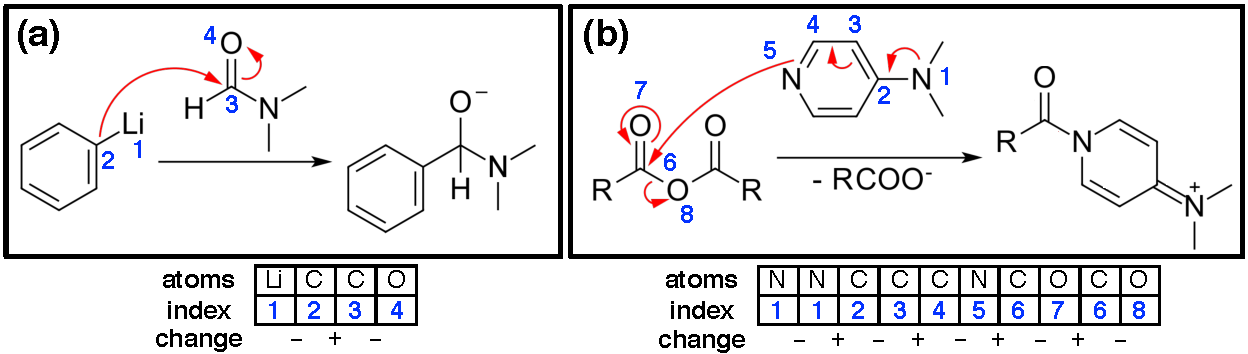
\includegraphics[width=\textwidth]{rxn_example}
\vspace{-3ex}
\caption{Two example reactions and their electron paths. In reaction (a), the reaction starts from an existing bond between Lithium (atom 1) and Carbon (atom 2). In reaction (b) the reaction starts from a lone-pair of electrons on Nitrogen (atom 1), which we represent formally as a bond with itself.}
\label{fig:example}
\end{figure*}

% KEY: separate assumptions from data processing
\section{Model}
In general, we want a model that, given an initial set of reactant molecules $\Mc_0$, produces a path of electron movements (some of which may be a `null' movement): $\Pc = (a_0, a_1, \ldots, a_{T-1})$ which, via a known deterministic function, yields a set of molecules $\Mc_1, \Mc_2, \ldots, \Mc_T$. 


% Because we do not know the true path $\Pc$, we can only receive a learning signal from the final predicted product molecules $\hat{\Mc}_T$ (compared to the true final molecules $\Mc_T$. This final predicted product is a deterministic (known) function $f$ of the initial molecules $\Mc_0$ and predicted actions $\hat{\Pc}$ (from $g$), as such $f(\Mc_0, \hat{\Pc}) = \hat{\Mc}_2, \ldots, \hat{\Mc}_T$.

% Ideally, we would like to learn the parameters of $g$, called $\theta$, to minimize the difference between the predicted final molecules $\hat{\Mc}_T$ and $\Mc_T$ (i.e., via some loss function $\ell$). However, we cannot resort to gradient-based techniques to learn $g$ because the inputs and outputs of $g$ are discrete objects, and the function $f$ producing $\hat{\Mc}_T$ is also discrete so the gradient $\frac{\partial \ell(\hat{\Mc}_T,\Mc_T)}{\partial \theta}$ does not exist. To solve this, we propose two types of models for this problem.

We propose to learn a parameterized distribution over electron movements: $p_\theta( \Pc \mid \Mc_0)$. We begin by describing the generative process (i.e., the forward pass) of $p_\theta$ and then describe how to train it.



\subsection{Generative process}
We factorize the distribution as follows:
\begin{align}
p_\theta(\Pc \mid \Mc_0) = p_\theta(a_{0} \mid \Mc_0) \prod_{t=1}^{T-1} p_\theta(a_{t} \mid a_{0:t-1}, \Mc_{0}) \nonumber
\end{align}
Note that we could not have factorized the above distribution via a Markov assumption as each individual path step $a_t$ depends not only on the previous path step $a_{t-1}$ and the previous molecule set $\Mc_{t-1}$, but also on the molecule set before this $\Mc_{t-2}$. This is because, as electron paths alternately break and form bonds we need to know whether the previous path step broke or removed bonds. As such, for generality, we condition the current path choice on all previous path choices.

As described in the previous section, if the three reaction assumptions above hold, then there are two types of electron movements that alternate: 1. movement that \emph{removes an existing bond}, and 2. movement that \emph{adds a new bond}. We can generalize assumption 3 by defining that atoms with free electrons have a self-bond. Thus, all reactions start by first selecting an atom, removing a bond (between two different atoms, or a self-bond), and alternately adding and removing bonds. %Figure~\ref{fig:example}(a) shows a reaction that starts from a bond between two different atoms and Figure~\ref{fig:example}(b) shows one starting from a bond between an atom and itself (i.e., an electron lone-pair). 

We parameterize remove-bond, add-bond, and start-atom steps in a similar way. Specifically, the functional form of a remove-bond step is described by the following equations:
\begin{align}
\Hb_{\Ac} \;&= f_{\Ac}(\Mc_t) \label{eq:rem_atom} \\
%\Hb_{\Bc} \;&= f_{\Bc}(\Mc_t, \Hb_{\Ac}) \label{eq:rem_bond} \\
p(a_t \mid a_{0:t-1}, \Mc_0) \;&= \mbox{softmax}(f_{\textrm{remove}}(\Hb_{\Ac}), a_{t-1}). \label{eq:rem_prob}  % HERERERE: think about if we allow bonds to go backwards (we could say it is very unlikely!)
\end{align}
Recall that $\Mc_t$ is a deterministic function of $\Mc_0$ and $a_{0:t-1}$.
Function $f_{\Ac}$ in eq.~\eqref{eq:rem_atom} takes a molecular graph and outputs a set of $d$-dimensional atom features $\Hb_{\Ac} \subseteq \mathcal{R}^{d \times |\Ac|}$ for each atom. In general $f_{\Ac}$ could be any deep graph model that uses the graph structure of $\Mc_t$ to get graph-isomorphic node features, usually via message-passing techniques \citep{gilmer2017neural}.
%In eq.~\eqref{eq:rem_bond}, $f_{\Bc}$ maps atom features $\Hb_{\Ac}$ to bond features $\Hb_{\Bc} \subseteq \mathcal{R}^{r \times (|\Ac|+1)|\Ac|/2}$, which could be as simple as a weighted-inner product or more flexible model such as a deep network. 
In eq.~\eqref{eq:rem_prob}, $f_{\textrm{remove}}$ followed by a $\mbox{softmax}$ function maps atom features $\Hb_{\Ac}$ to probabilities (which include a `null' stop action probability). The previous action $a_{t-1}$ (if it exists) is used to mask the resulting probabilities as follows:
\begin{align}
p(a \mid a_{0:t-1}, \Mc_0) \propto 
\begin{cases}
\mbox{softmax}(f_{\textrm{remove}}(\Hb_{\Ac})) & \mbox{if bond } (a_{t-1},a) \mbox{ exists in } \Mc_t \\
0 & \mbox{otherwise}. \nonumber
\end{cases}
\end{align}
For an add-bond step, we again use eq.~\eqref{eq:rem_atom} to obtain atom features $\Hb_{\Ac}$ and use a different function $f_{\textrm{add}}$ to produce add bond probabilities as follows: $p(a_t \mid a_{0:t-1}, \Mc_0) = \mbox{softmax}(f_{\textrm{add}}(\Hb_{\Ac}), a_{t-1})$
% \begin{align}
% \Hb_{\Ac} \;&= f_{\Ac}(\Mc_t) \label{eq:add_atom}  \\
% p(a_t \mid a_{0:t-1}, \Mc_0) \;&= \mbox{softmax}(f_{\textrm{add}}(\Hb_{\Ac}, a_{t-1})). \label{eq:add_prob}
% \end{align}
%The primary difference here is instead of a distribution over existing bonds, the distribution in eq.~\eqref{eq:add_prob} is over all possible atoms $\Ac$ (and a `null' action), as a bond may possibly form between any two atoms. 
Again we use the previous action $a_{t-1}$ to mask probabilities (here we only mask out the probability of adding a self-bond to the current atom).

Finally, in order to select the starting atom of a path we propose to model the initial probability as follows: $p(a_{0} \mid \Mc_0) = \mbox{softmax}(f_{\textrm{start}}(\Hb_{\Ac}))$.

\subsection{Training}
We can learn the parameters of $f_{\Ac},f_{\textrm{remove}},f_{\textrm{add}},f_{\textrm{start}}$, by minimizing the negative log-likelihood of the true path:
\begin{align}
\min_{f_{\Ac},f_{\textrm{remove}},f_{\textrm{add}},f_{\textrm{start}}} - \log p(a_0 \mid \Mc_0) - \sum_{t=1}^{T-1} \log p(a_t^* \mid a_{0:t-1}^*, \Mc_0) \nonumber
\end{align}
where $a_t^*,a_{0:t-1}^*$ are the true electron actions and the loss above describes the log probability given by the model to these true actions.

\subsection{Sampling}
Once trained we can sample chemically-valid paths via Algorithm~\ref{algo:valid_path}. 


\begin{wrapfigure}{R}{0.5\textwidth}
\begin{minipage}{0.5\textwidth}
\begin{algorithm}[H]
  \caption{Mapping to valid paths.}
  {\bf Input:}~~Predicted path $\hat{\Pc} = [\hat{a}_0, \hat{a}_1, \ldots, \hat{a}_{T-1}]$\\
  {\bf Input:}~~Molecule $\Mc_0$, remove flag $\texttt{F}_\textrm{remove} \!=\!1$
  
  \begin{algorithmic}[1]
  	\STATE Sample initial atom $\hat{a}_0 \sim p(a_0 \mid \Mc_0)$.
    \STATE $\hat{\Pc} = [\hat{a}_0]$%\ab^*_0]$
  	%\FORALL{atoms $\ab$ in molecule $\Mc_1$}
    %	\STATE 
    	%\STATE $i^* = \arg\min_{i \in \{1,\ldots,n\}} 
    %\ENDFOR
    \FORALL{$t$ from $1$ to $T-1$}
    	%\STATE Select predicted path $\hat{pb}_t$
    	\IF{$\texttt{F}_\textrm{remove} = 1$}
    		\STATE Sample atom $a \sim p(a_t \mid \hat{a}_{0:t-1}, \Mc_0)$% (or null action $\mathbf{0}$ if $t \neq T-1$) to $\hat{\ab}_t$, such that the bond $(\ab^*_{t-1}, \ab^*_{t})$ \emph{exists} in $\Mc_t$.
            \IF{$a$ is not `null'}
            	\STATE $\texttt{F}_\textrm{remove} = 0$
            \ENDIF
            \STATE Set $\Mc_t$ to molecule $\Mc_{t-1}$ but with bond $(\hat{a}_{t-1}, a)$ removed.
        \ELSE
        	\STATE Sample atom $a \sim p(a_t \mid \hat{a}_{0:t-1}, \Mc_0)$
            \IF{$a$ is not `null'}
            	\STATE $\texttt{F}_\textrm{remove} = 1$
            \ENDIF
            \STATE Set $\Mc_t$ to molecule $\Mc_{t-1}$ but with bond $(\hat{a}_{t-1}, a)$ added.
   		\ENDIF
        \STATE Set $\hat{a}_t = a$
        \STATE $\hat{\Pc} = [\hat{\Pc}, \hat{a}_t]$
    \ENDFOR
  \end{algorithmic}
  {\bf Output:}~~Valid path~$\hat{\Pc}$
  \label{algo:valid_path}
\end{algorithm}
\end{minipage}
\end{wrapfigure}


 




% While this assigns probabilities to discrete actions this can be a function of continuous embeddings of molecules as above. 

% To learn $g_\theta$, one idea is to sample a path $\Pc$ and apply it to our initial set of molecules $\Mc_0$. Using the known deterministic function $f$ we can produce a final predicted set of molecules $\hat{\Mc}_T$. However, even if we have a loss function $\ell(\hat{\Mc}_T,\Mc_T)$ we cannot use REBAR or RELAX to compute $\frac{\partial \ell(\hat{\Mc}_T,\Mc_T)}{\partial \theta}$ because $f$ is not stochastic. Maybe it's possible to make $f$ stochastic, then maybe it is possible to apply REBAR or RELAX.

% Another idea is to learn $g_\theta$ via maximum likelihood. Specifically, $g_\theta$ assigns some probability to all possible paths, so we can adjust $\theta$ to make the paths that lead to $\Mc_T$ more likely and those that do not less likely. I believe an efficient way to do this is to roll out only a few paths to produce $\hat{\Mc}_T$ (i.e., using the valid path sampling method using Algorithm~\ref{algo:valid_path}) and then update $\theta$ via $\frac{\partial \ell(\hat{\Mc}_T,\Mc_T)}{\partial \theta}$. Maybe Monte Carlo Tree Search could be useful here? I need to read more about this. 

% \subsection{Notes}
% In general I haven't given as much thought to a stochastic model. This is because ultimately we don't really want to give a chemist a distribution over electron paths, they want to know an actual prediction of electron movements. One could argue that this distribution might be a proxy for reaction `energy', but I don't think we need to learn a distribution to get this. We could make Algorithm 1 stochastic by instead of selecting the closest atom in steps 6 and 12, we select an atom with Gaussian probability given by the Euclidean distance between atoms in $\Mc_t$ and the predicted action $\hat{\ab}$. It's not clear to me whether this is a better or worse proxy for reaction energy.

% The main question is whether it will be easier to learn a stochastic function or two deterministic functions that give realistic electron paths. I think this boils down to (a) can we sample enough roll-outs to get a peaky distribution, (b) will learning both $g$ and $f$ lead to too much approximation error.



% We propose to learn a function $g: \Mc \rightarrow \Pc$. 

% Because we do not know the true path $\Pc$, we can only receive a learning signal from the final predicted product molecules $\hat{\Mc}_T$ (compared to the true final molecules $\Mc_T$. This final predicted product is a deterministic (known) function $f$ of the initial molecules $\Mc_0$ and predicted actions $\hat{\Pc}$ (from $g$), as such $f(\Mc_0, \hat{\Pc}) = \hat{\Mc}_2, \ldots, \hat{\Mc}_T$.

% Ideally, we would like to learn the parameters of $g$, called $\theta$, to minimize the difference between the predicted final molecules $\hat{\Mc}_T$ and $\Mc_T$ (i.e., via some loss function $\ell$). However, we cannot resort to gradient-based techniques to learn $g$ because the inputs and outputs of $g$ are discrete objects, and the function $f$ producing $\hat{\Mc}_T$ is also discrete so the gradient $\frac{\partial \ell(\hat{\Mc}_T,\Mc_T)}{\partial \theta}$ does not exist. To solve this, we propose two types of models for this problem.

% \paragraph{Deterministic.}
% Instead, we assume we have continuous mappings from molecules $\Mc$ to vectors $\mb$ and paths $\Pc$ to matrices $\Pb$. We propose to learn continuous functions $g_\theta: \mb \rightarrow \Pb$ and $f_\phi: \mb, \Pb \rightarrow \mb, \ldots, \mb$. Then we can compute derivatives of a loss function $\ell(\hat{\mb}_T,\mb_T)$ with respect to parameters $\theta$ as follows. Let $\hat{\mb}_T = [f(\mb_1,g(\mb_1))]_T$. Then our gradient is $\frac{\partial \ell(\hat{\mb}_T,\mb_T)}{\partial \theta} = \frac{\partial \ell(\hat{\mb}_T,\mb_T)}{\partial f}\frac{\partial f}{\partial g}\frac{\partial g}{\partial \theta}$.

% Note that now, $f_\phi$ is unknown. So we propose to learn it given observed traces: $(\mb_1,\Pb,\mb_2,\ldots,\mb_T)$. For simplicity define $\Mb_{2:T} = [\mb_2,\ldots,\mb_T]$, and $f(\mb_1,\Pb) = \hat{\Mb}_{2:T}$. Then, given a loss function $l(\hat{\Mb}_{2:T},\Mb_{2:T})$ we can learn the parameters of $f$, called $\phi$ via the gradient $\frac{\partial l(\hat{\Mb}_{2:T},\Mb_{2:T})}{\partial \phi} = \frac{\partial l(\hat{\Mb}_{2:T},\Mb_{2:T})}{\partial f} \frac{\partial f}{\partial \phi}$.

% In order to ensure that $g_\theta$ produces paths $\hat{\Pb}$ that are valid (i.e., that alternately remove and add bonds) we propose to take a predicted path $\hat{\Pb}$ and map it to a valid path $\Pb^*$ as described in Algorithm~\ref{algo:valid_path}. Given a valid path, we propose a loss function $L(\hat{\Pb},\Pb^*)$ and learn $g_\theta$ to minimize this loss via $\frac{\partial L(\hat{\Pb},\Pb^*)}{\partial \theta} = \frac{\partial L(\hat{\Pb},\Pb^*)}{\partial g} \frac{\partial g}{\partial \theta}$.



% %another loss function 
% %Finally, one last appealing property of this model is that if similar molecules have similar continuous representations embeddings then the functions $g_\theta, f_\phi$ allow us to generalize to similar molecules we have not seen before.
% Function $f_\phi$ could be an RNN and $g_\theta$ could be a fully connected network. We could consider an alternative $g_\theta$ that is conditioned on previous states which could be an RNN. 



% \paragraph{Stochastic.}

%Given a learned distribution we could sample valid paths using Algorithm~\ref{algo:valid_path}. We could use a model similar to DRAW. Maybe it is possible to not learn $f$ and instead use a dynamic programming algorithm to update $g_\theta$. Otherwise, we could learn $f$ as a stochastic function over discrete states. In general I haven't given as much thought to a stochastic model.
%Note that this distribution is not Markov as we need to know if the previous two electron movement added or removed a bond, in order to determine whether we need to consider only existing bonds or not. We could use a model similar to DRAW and mask all samples so agree with these constraints.




% TODO:
% - write intuitive idea
% - formalize variables
% - wait a long time until writing objective
% - wait even longer to write optimization

\bibliography{bibliography}
\bibliographystyle{plainnat}


\end{document}
